%%% A Sample Thesis Written Using LaTeX.
%%%
%%% C.M. Connelly <cmc@math.hmc.edu>
%%%
%%%  $Id: sample-thesis-report.tex 205 2006-04-15 01:17:39Z cmc $

%%% Copyright (C) 2004-2005 Claire M. Connelly and 
%%% the Department of Mathematics, Harvey Mudd College.
%%%
%%% This file is part of the sample thesis document provided to HMC
%%% mathematics students.
%%%
%%% See the COPYING document, which should accompany this
%%% distribution, for information about distribution and modification
%%% of the document and its components.


%%% The top part of your document is called the preamble.  You supply
%%% some basic information about the document (such as its title and
%%% author) in a form that LaTeX can understand here.

%%% You can also load additional LaTeX packages, or style files, that
%%% affect the way that the document is laid out, typeset, or supply
%%% additional commands or environments.

%%% The preamble can also be used to define your own commands and
%%% environments, set some constants that will be used throughout your
%%% document, and so on.

%%% As you may have guessed, LaTeX's comment character is the percent
%%% sign.  Any line that starts with a % will be ignored.  You can
%%% also use the comment character to add comments to the end of a
%%% line that will be parsed by TeX.


%%% The first active line in your LaTeX document is the \documentclass
%%% command, which loads a LaTeX class file.  Class files generally
%%% define the appearance of a document, and include a variety of
%%% structural commands.

%%% Clinic reports use the clinic class, which should be located
%%% somewhere in TeX's search path.

\documentclass{hmcthesis}

%%% Other packages needed by your document may be loaded here.
\usepackage{url}              % For formatting URLs and other web or
                              % file references.
\usepackage{mflogo}           % Provides the METAFONT logo.
\usepackage{booktabs}         % Publication-quality tables.
\usepackage{natbib}           % Provides some nice citation and
                              % bibliography formatting commands.
\bibpunct[:~]{(}{)}{;}{a}{,}{,~} % Set some defaults for bibliographic
                                 % punctuation used by natbib.sty.
\usepackage{verbatim}
\usepackage{graphicx}
\usepackage{calc}
\usepackage{subfig}
\usepackage{textcomp}
\usepackage[plainpages=false,pdfpagelabels]{hyperref}

\includeonly{%
%%% Chapter 1
introduction
%%% Chapter 2
,structured-writing
%%% Chapter 3
,mathematics
%%% Chapter 4
,figs-and-tables
%%% Chapter 5
,typesetting
%%% Chapter 6
,tips-and-tricks
%%% Chapter 7
,resources
%%% Chapter 8
,books
%%% Appendix
,versions
}


%%% Provide additional context around errors. 
\setcounter{errorcontextlines}{1000}

%%% Information about this document.

%%% I find it most useful to put identifying information about a
%%% document near the top of the preamble.  Technically, this
%%% information must precede the \maketitle command, which often
%%% appears immediately after the beginning of the document 
%%% environment.  Placing it near the top of the document makes it
%%% easier to identify the document, and keeps it out from getting
%%% mixed up with the real meat of the document.

%%% So, some questions.

%% What is the title of your report?
\title{A Sample Thesis Report, Showing the Reader the Wonder of
  Formatting Documents Using \LaTeX}

%% Your name (or names, if you are writing a joint thesis).  (Separate
%% names with \and.)
\author{Claire Connelly}

%% What is your faculty advisor's name?  (Again, separate names with
%% \and, if necessary.)
\advisor{Melissa O'Neill}

%% Second reader's name?
\reader{Second Reader}

%% The year in which you are submitting your thesis.
\thesisyear{2006}

%% The month in which you are submitting your thesis (if not May).
% \thesismonth{December}

%%% End of information section.

%%% New commands and environments.

%%% You can define your own commands and environments here.  If you
%%% have a lot of material here, you might want to consider splitting
%%% the commands and environments into a separate ``style'' file that
%%% you load with \usepackage.

\newcommand{\coolcommand}[1]{#1 is cool.} % Lets everyone know that
                                % the person or thing that you provide
                                % as the argument to the command is
                                % cool.

%%% You probably won't want any of the following commands, which are
%%% here to allow various the names of commands, make examples typeset
%%% properly, and so on.  You can, of course, use them as examples for
%%% your own user-defined commands.
                                                                               
\newcommand{\bslash}{\symbol{'134}}%backslash
\newcommand{\bsl}{{\texttt{\bslash}}}
\newcommand{\com}[1]{\bsl\texttt{#1}\xspace}
\newcommand{\file}[1]{\texttt{#1}\xspace}

\newcommand{\pdftex}{PDF\tex}
\newcommand{\pdflatex}{PDF\latex}
\newcommand{\acronym}[1]{\textsc{#1}\xspace}
\newcommand{\key}[1]{\textsf{\emph{#1}}\xspace}
\newcommand{\class}[1]{\textsf{#1}\xspace}
\newcommand{\package}[1]{\textsf{#1}\xspace}
\newcommand{\env}[1]{\texttt{#1}\xspace}
\newcommand{\prog}[1]{\texttt{#1}\xspace}
\newcommand{\command}[1]{\texttt{\bsl{}#1}\xspace}
\newcommand{\ctt}{\texttt{comp.text.tex}\xspace}
\newcommand{\tex}{\TeX\xspace}
\newcommand{\latex}{\LaTeX\xspace}
\newcommand{\host}[1]{\textsf{#1}\xspace}
                                                                                


\newcounter{cms}

%%% Some theorem-like command definitions.

%%% The \newtheorem command comes from the amsthm package.  That
%%% package is loaded by the class file.

\newtheorem{thm}{Theorem}[chapter]
\newtheorem{Theo1}{Theorem}[chapter]
\newtheorem{Theo2}{Theorem}[chapter]
\newtheorem{Lemma}{Lemma}[chapter]


%%% If you find that some words in your document are being hyphenated
%%% incorrectly, you can specify the correct hyphenation using the
%%% \hyphenation command.  Note that words are separated by
%%% whitespace, as shown below.

\hyphenation{ap-pen-dix wer-ther-i-an}


%%% The start of the document!

%% The document environment is the main environment in any LaTeX
%% document.  It contains other environments, as well as your text.

\begin{document}

%%% The front matter of a large document includes the title page or
%%% pages, tables of contents, lists of figures or tables, and so on,
%%% your abstract, a preface or introduction, and so on.  It's
%%% delineated with the \frontmatter command.
\frontmatter

%%% One of the things that the \frontmatter does is make page
%%% numbers appear as lowercase Roman numerals---i, vi, xii, and so
%%% on.

%%% The first thing in the front matter is your title page.  The title
%%% page is formatted by commands in the document class file, so you
%%% don't need to worry about what it looks like -- just putting the
%%% \maketitle command in your document (and filling in the necessary
%%% information for the identification commands above) is enough.
\maketitle


%%% Abstract

%%% Your abstract should be a \emph{brief} summary of the contents
%%% of your report.  Don't go into excruciating detail
%%% here---there's plenty of room for that later.

\begin{abstract}
  This document is a sample of what can be done with \LaTeX.  In
  addition to demonstrating the features of the \textsf{hmcclinic}
  and \textsf{hmcthesis} classes, we hope to provide useful and
  clear examples of not only what can be done, but how best to do it.
\end{abstract}


%%% Acknowledgments (Optional).

%%% If you want to thank someone for their influence on your life or
%%% your work, here's where you'd do it.

\begin{acknowledgments}
  To Melissa O'Neill, Lesley Ward, Michael Raugh, Barbara Schade,
  and Jeremy Rouse, without whom this document would not exist in
  its present form.
\end{acknowledgments}




%%% Table of Contents, List of Figures, and List of Tables.
%%% 
%%% If you don't have any figures or tables in your report, you can
%%% comment out the appropriate command.

\tableofcontents
\listoffigures
\listoftables


%%% End of the front matter.

%%% Beginnning of the main matter.

%% The main part of your report consists of normal, numbered
%% chapters.  The main matter is opened with the \mainmatter command.
\mainmatter


%%% Content.

%%% For smaller documents---especially those you're writing by
%%% yourself---you might write your entire report using a single LaTeX
%%% source file.  For larger documents, we recommend that you split
%%% the source file into several separate, smaller files.  The smaller
%%% files are ``included'' into your main, or ``master'' document
%%% using \include commands.

%%% Splitting your source has several advantages.  One, it allows you
%%% to have more than one person working on different parts of the
%%% document at the same time (although we still recommend that you
%%% use CVS or a similar revision-control system!).  Two, smaller
%%% document chunks allow you to reorganize your document more easily.
%%% If your decide that Chapter 8 would be better as Chapter 4, all
%%% you have to do is swap the \include commands around.  For that
%%% reason, you may want to consider giving your separate chapters
%%% meaningful names rather than calling them ``chapter1'',
%%% ``chapter2'', and so on.

%%% Finally, splitting the document allows you to concentrate on a
%%% particular section without being distracted by other
%%% sections---all you have to do is comment out the \include line for
%%% the sections you're not working on.  This technique can be
%%% especially useful when you're trying to track down a problem by
%%% allowing you to easily locate the file with the problem and
%%% rule out the other sections.

%%% In our example document, we're going to define a slew of chapters,
%%% each of which has some useful information about writing Clinic
%%% reports or using LaTeX.

%%% Chapter 1
%%% Copyright (C) 2004 Claire M. Connelly and 
%%% the Department of Mathematics, Harvey Mudd College.
%%%
%%% This file is part of the sample thesis document provided to HMC
%%% mathematics students.
%%%
%%% See the COPYING document, which should accompany this
%%% distribution, for information about distribution and modification
%%% of the document and its components.

\chapter{Introduction}%
\label{sec:introduction}


\section{Sponsors} \label{background}

Our project is unique because we have two independent stakeholders (IES and PilotCity) who have different but connected areas of interest.
\begin{itemize}
    \item \textbf{Institute of Education Sciences (IES)} is the statistics, research, and evaluation arm of the U.S. Department of Education. Their mission is to provide scientific evidence on which to ground education practice and policy and to share this information in formats that are useful and accessible to educators, parents, policymakers, researchers, and the public (Institute of Education Science Website, 2019).
    \item \textbf{PilotCity}, on the other hand, is a startup that was created to help transform small to medium sized cities into innovation engines by converting local high school classrooms into workforce incubators. The motivation behind PilotCity is to generate talent within a city, rather than attract it from the outside. To realize this vision, PilotCity connects local high schools and employers thereby empowering students at an early age and promoting the idea of project based learning.
\end{itemize}

\section{Problem Statements}

\subsection{PilotCity}

In the past, PilotCity has manually performed logistical tasks like recruiting, signing up teachers and employers and matching employers to classrooms. However, manual program delivery is a bottleneck to PilotCity's capacity to scale and thus PilotCity aims to automate most of their processes like enrollment and matchmaking with the aid of the Harvey Mudd Clinic program. Our team has thereby been tasked with improving user engagement and scalability of PilotCity programming by helping design and create a web interface that students, teachers and employers can better interface with as well as building a recommender system to facilitate matching employers to high school classrooms. 

\subsection{IES}

While we help facilitate PilotCity programming, we are also tasked by IES to research and come up with new ways to gain insights on educational priorities and approaches from uncurated educational resources like course websites, syllabi and teacher resumes. To fulfill this task, we decided to employ topic modeling techniques on a collection of syllabi pertaining to a college to make inferences on the nature of a college's curriculum. This exploration was motivated by work by Sekiya et al who present a similar investigation to ours but with a slightly different angle and scope (Sekiya, Matsuda, \& Yamaguchi, 2017). Rather than looking at all course subjects across time at one school, they narrow the focus to computer science curriculum across multiple schools within the same time frame. Furthermore, rather than having to train a topic model themselves, they leverage the pre-existing CS2013 Body of Knowledge (BOK), produced by the ACM and IEEE Computer Society and detailing the 18 primary topics in Computer Science curriculum as of 2013. Sekiya et al. used those 18 topics to train a simplified, supervised Latent Dirichlet Allocation model (ssLDA) which then output, for a given unseen computer science syllabus, how much each of those 18 core topics were represented. However, since we lack predefined topics, our work involves training unsupervised topic models to discover the core topics across all disciplines at Las Positas College in Livermore, California.



%% TODO
%%
%% Add sections addressing
%%
%%  More about specific things that we cover
%%
%%  Lecturing about how to do various things
%%
%%    naming chapter filess sensibly
%%
%%  Contents of the class file and example document


%%% Local Variables: 
%%% mode: latex
%%% TeX-master: "master"
%%% End: 


%%% Chapter 2
\include{structured-writing}

%%% Chapter 3

\include{mathematics}

%%% Chapter 4

\include{figs-and-tables}

%%% Chapter 5

\include{typesetting}

%%% Chapter 6

%%% Copyright (C) 2004 Claire M. Connelly and 
%%% the Department of Mathematics, Harvey Mudd College.
%%%
%%% This file is part of the sample thesis document provided to HMC
%%% mathematics students.
%%%
%%% See the COPYING document, which should accompany this
%%% distribution, for information about distribution and modification
%%% of the document and its components.

\chapter{Tips and Tricks}

\latex is a very complicated and powerful language.  As a result,
there are many sneaky aspects to it that will cause you problems if
you don't know about them.  This chapter covers some of these tricky
bits.


\section{Special Characters}%
\label{sec:special-chars}

\tex and \latex have a number of ``special'' characters that are
reserved for use by the language.  Using these characters in your
writing requires you to do a bit of extra work, as shown in
Table~\ref{tab:special-chars}.

\begin{table}
\begin{tabular}{llll}
\toprule
\multicolumn{2}{l}{Character}   & Function     & To Typeset\\
\midrule
\#          & octothorp      & Macro parameter character  & \verb+\#+\\
\$          & dollar sign    & Start/end inline math mode & \verb+\$+\\
\%          & percent sign   & Comment character          & \verb+\%+\\
\&          & ampersand      & Column separator           & \verb+\&+\\
\_          & underscore     & Subscripts, as in $x_2$    & \verb+\_+\\
\{, \}      & braces         & Parameters                 & \verb+\{, \}+\\
\~{}        & tilde          & Nonbreaking space          & \verb+\~{}+ \\
\^{}        & caret          & Superscripts, as in $x^2$  & \verb+\^{}+\\
\verb+\+    & backslash      & Starts commands   & \command{verb}\verb+|\|+ \\
\bottomrule
\end{tabular}
\caption[Special characters in \latex]{Special characters in \latex.}%
\label{tab:special-chars}
\end{table}


\section{Accents}

There are a variety of commands for producing diacritical accents, as in
\begin{quote}
  Paul Erd\H{o}s s'est reveill\'{e} t\^{o}t pour enseigner le
  fran\c{c}ais \`{a} son fr\`{e}re et sa s\oe{}ur.
\end{quote}

See Section~2.4.7 in \emph{Math into \LaTeX} \citep{gratzer-mil} for
information about accents (and some handy charts!).


\section{Comments and Spacing}

You can add comments to your source file that won't appear in your
typeset document by starting them with a \verb+%+.  Any line that
starts with a \verb+%+ will be ``commented out'', and won't be
interpreted.  You can also add a \verb+%+ at the end of a line, with
or without text, and it will make the end of the line (including the
linebreak!) disappear.

For example,
\begin{quote}
\begin{verbatim}
% This line is a comment line.
This line is not a comment line.

This line has a comment at the end%
% This line should be invisible.
of the line.
\end{verbatim}
\end{quote}
will typeset as
\begin{quote}
% This line is a comment line.
This line is not a comment line.

This line has a comment at the end%
% This line should be invisible.
of the line.
\end{quote}

Notice the lack of a space in ``endof'' on the last line of the
typeset output.  \tex expects to find  a carriage-return character at the end
of a line, and interprets that carriage return as an interword space.
If you comment out the end of a line, you also comment out the
carriage return on that line, and you'll have words run into one
another unless you have a space before the \verb+%+.

\tex collapses multiple spaces into one, and ignores whitespace at the
beginning of a line.  Thus
\begin{quote}
\begin{verbatim}
No spaces.

    Five spaces.

    A tab.
\end{verbatim}
\end{quote}
typesets as
\begin{quote}
No spaces.

    Five spaces.

    A tab.
\end{quote}

(The lines are indented because they are at the start of a paragraph.
You can suppress paragraph indentation with \command{noindent}.)

Paragraphs are delimited by two carriage returns (with or without
whitespace between them).


\section{Quotes and Dashes}

Because \tex was designed to do high-quality typesetting, it cares
about which quotation mark and dash you're using, and requires you to
specify the correct punctuation (although most text editors with
special \tex modes will do the substitution for you).

Open and close double quotes---`` and ''---are created by typing
\verb+``+ and \verb+''+, respectively.  The double-quote mark,
\verb+"+, is typeset as " (and is useful for abbreviating ``inches'',
as in 36").

Single-quotes, ` and ', are typed with \verb+`+ and \verb+'+.

There are three basic forms of dashes:
\begin{enumerate}
\item The hyphen, -, is typed as a single dash, \verb+-+
\item The en dash, --, is typed as two dashes, \verb+--+
\item The em dash, ---, is typed as three dashes, \verb+---+
\end{enumerate}

Hyphens are used in hyphenated words, as in ``high-quality''.  En
dashes are used to indicate ranges, as in ``there are 35--50 of
them''; balanced relationships, as in ``U.S.--European agreements'';
and for extended hyphenated phrases, such as ``reddish-green--colored
item''.   Em dashes are used to separate independent phrases, as in
``John believed---honestly believed---that he was right''; and to
indicate interruptions in dialogue, as in
\begin{quotation}
  ``I hear you---''

  ``No, you don't!''
\end{quotation}

Note that you shouldn't type spaces around any of these dashes---they
run directly against the words on either side, as in \verb+35--50+.


\section{Controlling Pagination}%
\label{sec:pagination}

Sometimes you may need to override \LaTeX's choices for line or page
breaks.  The \com{pagebreak} command causes \LaTeX\ to start a new
page immediately after the command appears.  The \verb|\\| command can
be used to tell \LaTeX\ where to break a line.

In general, you should let \LaTeX\ have its way, especially if your
document is going to be published by someone else, as they will
undoubtedly have many changes that will have to be made before your
document works for them.  If you do need to tinker with your
document's layout, you should avoid doing so until you're very nearly
done.  If you go back and add or remove text after forcing \LaTeX\ to
do your will, you may find that new blank spaces appear as a result of
your changes.

George Gr\"{a}tzer's \emph{Math into \LaTeX} \citeyearpar{gratzer-mil}
includes a chapter on preparing books that covers this topic in depth.


\section{Using Graphics with \pdftex}%
\label{sec:pdftex-graphics}

\pdftex supports PDF and JPEG as native graphic file formats.  EPS is
not directly supported---to use EPS figures with \pdftex, you must
first convert your EPS files to PDF.  

If you're using a graphics program such as Adobe Illustrator to
prepare your figures, just save them as PDF instead of (or in addition
to) EPS.

If you don't have access to the tool you used to create your images,
but you still need to convert them, you can use the program
\prog{epstopdf}.

\prog{epstopdf} writes to standard output by default, so you'll have
to redirect the output to a file, as in
\begin{quote}
\begin{verbatim}
unix% epstopdf foo.eps > foo.pdf
\end{verbatim}
\end{quote}

To convert a whole slew of files, you could use a command such as the
following (with the \prog{csh}):
\begin{quote}
\begin{verbatim}
unix% foreach f ( `find . -type f -name '*.eps'`)
foreach? eps2pdf $f -o=$f:r.pdf
foreach? end
\end{verbatim}
\end{quote}


\section{Fonts Look Fuzzy in PostScript or PDF Files}%
\label{sec:fuzzy-fonts}

When Donald~E. Knuth originally wrote \tex, most typesetting was done
by trained typesetters using expensive equipment to cast molten lead
into runs of type.  Knuth created his own font family, Computer
Modern, by writing a tool called \MF{}.  \MF{} reads in programs that
define various aspects of every character in a font, and generates
bitmap representations of those characters at a particular resolution,
ready for printing.

Unfortunately, bitmaps with resolutions suited for printing look
terrible on screen.  The solution is to use Type~1 PostScript fonts
instead of bitmaps. If you're using \pdftex (or \pdflatex), you get
Type~1 fonts without having to do anything special (but see
Section~\ref{sec:pdftex-graphics}).

If you're using \prog{dvips} to get PostScript as an intermediate step
(using \prog{ps2pdf} or Acrobat Distiller to get PDF), you can force
\prog{dvips} to use Type~1 fonts by specifying the \prog{-Ppdf} flag,
as in
\begin{quote}
\begin{verbatim}
unix% dvips -Ppdf foo.dvi -o foo.ps
\end{verbatim}
\end{quote}


\section{Debugging}

One of the trickiest things about using \latex is interpreting
\latex's sometimes cryptic error messages.

In particular, the line numbers that \latex reports are often not the
line numbers where the problem \emph{is}, but the line numbers where
\latex noticed there was a problem.

One useful way of getting a bit more context to help you understand
the problem is to put the line
\begin{quote}
\begin{verbatim}
\setcounter{errorcontextlines}{1000}
\end{verbatim}
\end{quote}
in the preamble of your document, which will provide you with a
(perhaps excessive) amount of context for an error.

The most common errors are
\begin{itemize}
\item Using one of the special characters (see
Section~\ref{sec:special-chars})
\item Leaving off or mismatching a brace or bracket
\item Leaving out or swapping arguments to a command or environment
\end{itemize}

If you've tried everything and you can't find the source of an error
message, try the following procedure:
\begin{enumerate}
\item Create a new file, and copy your preamble into it, followed by
  an empty \env{document} environment
\item Add a word to the \env{document} environment so that \tex will
  have something to typeset
\item Try typesetting the new document---if you have an error, the
  problem is in your preamble
\item If the document typesets, get rid of the single word you'd put
  in the \env{document} environment, copy half of your original
  document's body into the new file, and typeset that
\item If you see your error, then continue halving the document until
  you narrow it down to the problem section
\item If you don't see your error, try the other half
\end{enumerate}

\subsection{The \protect\env{comment} Environment}

If you don't want to go through the process of copying your document,
you can also use the \env{comment} environment, which allows you to
``comment out'' anything between the begin and end environment
commands.  The \env{comment} environment is provided by the
\package{verbatim} package, which also defines new versions of the
\env{verbatim} and \env{verbatim*} environments.

\subsection{The \protect\command{includeonly} Command}

If you've written your document in such a way that each chapter or
other significant subdivision is stored in a separate file and
included in your master document with an \command{include} command,
then you can also use the \command{includeonly} command to limit the
parts of your document that will be typeset to some subset.

\command{includeonly} takes as its argument a comma-separated list of
files that are \command{include}d in your document.  If you place each
item on a separate line, you can comment and comment those lines to
control which files are included in a \latex run.  For example,
\begin{quote}
\begin{verbatim}
\includeonly{
a,
% b,
% c,
d}
\end{verbatim}
\end{quote}
will allow you to typeset the contents of the files \file{a} and
\file{d}, without typesetting the contents of \file{b} and \file{c}.
A nice side-effect is that the auxilliary files for these files are
not changed, so that references to labels in the files not being
typeset will still be expanded in the files that are typeset.  (If the
pagination changes, of course, any \command{pageref} commands will be
incorrect; the same applies if any additional structural commands are
added at the same level as the topmost level in the excluded
files---that is, if you add a new chapter in a file called \file{aa}
between the line that includes \file{a} and \file{b}, the chapter
numbers will be incremented for the typeset files but not for the
files you're not typesetting.

%%% Local Variables: 
%%% mode: latex
%%% TeX-master: "master"
%%% End: 


%%% Chapter 7

%%% Copyright (C) 2004 Claire M. Connelly and 
%%% the Department of Mathematics, Harvey Mudd College.
%%%
%%% This file is part of the sample thesis document provided to HMC
%%% mathematics students.
%%%
%%% See the COPYING document, which should accompany this
%%% distribution, for information about distribution and modification
%%% of the document and its components.

\chapter{Resources}

There are lots of great resources available for using \tex and \latex.
Here are a few (there are also links available online at\\
\url{http://www.math.hmc.edu/computing/support/tex/}).


\section{Online Documentation}%
\label{sec:online-docs}

Much of the documentation for \tex and \latex is available online, as
part of the \tex system.  te\tex, the \tex system installed on the
mathematics department's computers, includes a script called
\prog{texdoc} to access this documentation.  All you have to do is
type \prog{texdoc} followed by a string that you believe is the name
of the document you're looking for.  For example, \prog{texdoc
  booktabs} will give you the documentation for the \package{booktabs}
package that I used to create the tables in this document.

Unfortunately, \prog{texdoc} only works for documentation that is
sensibly named.  The authors of the \package{graphics} package, for
instance, called their manual \file{grfguide}.  Still others decided
that \file{manual} was a good name for their manual (after all, it's
the only \emph{manual} in their distribution).

Sometimes you can find documentation using the \prog{locate} command,
which lists all the files on your system that match a string that you
provide.  For example, you could find \file{grfguide} by trying
\prog{locate graphics} and \prog{grep}ping out the results with
\file{texmf} in them, and passing that list to another \prog{grep} for
the string \file{doc}:
\begin{quote}
\begin{verbatim}
unix% locate graphics | grep texmf | grep doc
\end{verbatim}
\end{quote}

Another hard to find, but very useful, document, is the ``User's Guide
for the \package{amsmath} Package'' \citeyearpar{amsmath-doc}, which
is called \file{amsldoc}.

\subsection{\protect\command{texdoctk}}

Our current te\tex installation includes the \prog{texdoctk} program,
which gives you a graphical window into the documentation installed on
the system.  You start \prog{texdoctk} by typing its name at a shell
prompt.  A window (Figure~\ref{fig:texdoctk}) will appear with buttons
corresponding to broad categories of documentation; clicking on one
will open another dialog box with the titles of available
documentation (with the names of the actual packages in parentheses).

\begin{figure}[htbp]
  \centering
  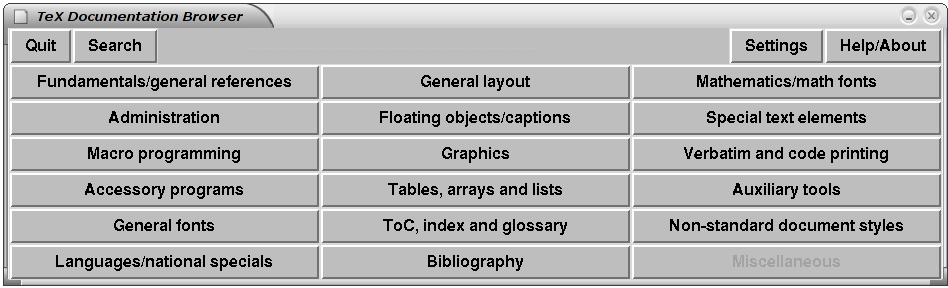
\includegraphics[width=\textwidth-2cm,keepaspectratio=true]{texdoctk}
  \caption[\protect\prog{texdoctk} main window]{\prog{texdoctk} main window.}
  \label{fig:texdoctk}
\end{figure}


\section{UK-TUG FAQ}

The primary list of frequently asked questions in the \tex world is
the UK TUG FAQ, available at
\url{http://www.tex.ac.uk/cgi-bin/texfaq2html}.  If you're not sure
how to do something, or you've got a problem that you're pretty sure
isn't being caused by a typo, check here first.


\section{\ctt}

If you can't find an answer in the UK-TUG FAQ, then your next step is
to check \ctt, the Usenet newsgroup devoted to \tex and \latex.
Chances are, whatever your problem is, someone else already had it,
asked about it on \texttt{c.t.t}, and got an answer.  Thanks to Google, Usenet's
past is preserved in an easily searchable format.  Go to Google Groups
(\url{http://groups.google.com/}), type in some search terms, and
check out the answers.  (If you specify \texttt{group:comp.text.tex}
at the end of your search terms, you'll only see results from \ctt.)


%%% Local Variables: 
%%% mode: latex
%%% TeX-master: "master"
%%% End: 



%%% Chapter 8

%%% Copyright (C) 2004 Claire M. Connelly and 
%%% the Department of Mathematics, Harvey Mudd College.
%%%
%%% This file is part of the sample thesis document provided to HMC
%%% mathematics students.
%%%
%%% See the COPYING document, which should accompany this
%%% distribution, for information about distribution and modification
%%% of the document and its components.

\chapter{Books}

\url{http://www.math.hmc.edu/computing/support/tex/} has some brief
reviews of a number of significant books about \tex and \latex.

My pick for the best introductory/reference book is the third edition
of George Gr\"{a}tzer's \emph{Math into \latex{}}
\citeyearpar{gratzer-mil}.\footnote{Which I edited.}  It's the only book I'm
aware of that discusses the latest version of AMS\latex in depth.  It
also has excellent reference tables and a thorough index.

Another book I highly recommend is Lyn Dupr\'{e}'s \emph{BUGS in
  Writing} \citeyearpar{dupre-bugs}.  Dupr\'{e} is one of Addison Wesley's
senior editors, and has edited many of the most significant books
published by Addison Wesley.  \emph{BUGS} is an accessible guide to
writing clearly and effectively.  It's the kind of book you leave in
the bathroom so you'll always have something interesting and amusing
to read.  Learning how to write better is almost a byproduct!

If you get serious about typesetting, and want to start doing some
fancy page design or want to be sure you're using the right kind of
type, Robert Bringhurst's \emph{The Elements of Typographic Style}
\citeyearpar{bringhurst-elements} will show you the way.





%%% Appendices.

%%% Appendices are just like chapters, only they're generally lettered
%%% rather than numbered (although that depends on your document
%%% class, of course).

%%% The appendices are delineated with the \appendix command.
%%% Individual appendices are begun with the standard \chapter or
%%% \section commands.  In our example, we'll \include them just as we
%%% did other chapters.
\appendix

\chapter{Versions of the Sample Thesis/Clinic Report}
\label{ch:previous_versions}

This document is based, in part, on earlier versions of sample
Clinic reports and sample theses.  Some material from those versions
is included nearly intact in this document, whereas other material
has been written from scratch or adapted from other sources.

The authors of the present work would like to acknowledge and thank
Professor Lesley Ward for her original sample thesis report, created
in 1999.  She and Jeremy Rouse (HMC~2003) revised that document in
the year 2000.

The current version of the document is based on the updated sample
thesis created in 2003 by Claire~M. Connelly, the Department of
Mathematics Systems Administrator.  The original sample Clinic
report was based on this sample thesis document.

In 2005, Claire merged the sample thesis and sample Clinic reports,
making maintenance and distribution a bit easier.


\section{Comments, Problems, and Updates}
\label{sec:feedback}

The department is eager to receive feedback from users of the sample
document so that we can improve it.  We are especially interested in
any problems that you may have in compiling the document, but
advice, questions, and updates to the content are also welcome.

Please send such comments and ``bug reports'' to us at
\textsf{latex@math.hmc.edu}.  If possible, please tell us where you
downloaded the document's source code, and what version and date are
noted in the master file for the document you're working with.





%%% Back matter.

%%% The back matter of a document is where the bibliography and index
%%% are defined.  It starts, not surprisingly, with the \backmatter
%%% command. 

\backmatter


%%% Bibliography.

%%% BibTeX is the tool to use for citations and layout of your
%%% bibliography.  Instead of having to type ``[5]'' or ``(Jones,
%%% 1968)'' (and keep track of which citation is which and renumber
%%% them as you add more references to your bibilography), you use
%%% special commands that allow BibTeX and LaTeX to automatically put
%%% the correct information in the right place.

%%% Depending on your field, it may or may not be appropriate to list
%%% references for which you haven't included specific citations.  If
%%% your field sanctions such practices, or if you just want to get an
%%% idea of what you have in your bibliography file, you can include
%%% everything with the \nocite{*} command.
\nocite{*} 


%%% The appearance of your bibliography and citations in your text are
%%% defined by a combination of any bibliography-related LaTeX
%%% packages (such as natbib, harvard, or chicago) and the particular
%%% bibliography style file that you load with the \bibliographystyle
%%% command.  Bibliography-style files end in .bst; you can find them
%%% by searching your file system using whatever tools you have for
%%% doing searches.  (On most modern Unices, ``locate .bst'' will give
%%% you an idea of what's available.)

\bibliographystyle{plainnat}

%%% The particular bibliography data file or files that you want to
%%% use are specified with the \bibliography file.  Multiple files are
%%% separated by commas.

%%% You might want to use multiple bibliography (or ``bib'') files if
%%% you had a master bib file containing references you use again and
%%% again, and another containing only records for references for a
%%% particular project.

%%% Many people create a single, large bib file that they use for
%%% everything they write.  That approach requires you to \cite every
%%% reference that you want to use in your document -- using
%%% \nocite{*} with a huge bibliography database will give you a large
%%% bibliography containing many references you haven't consulted for
%%% your particular document!

\bibliography{sample}


%%% Glossary or Index.

%%% If you were going to include a glossary or index in your document,
%%% the relevant commands would appear here.

%%% If you think that you would like to include such features, talk
%%% with someone who's worked with LaTeX a lot very early in your
%%% writing process.  These commands require you to do a bit of
%%% thinking about what you would want to index or gloss in advance --
%%% going back though a completed document to add \index commands is
%%% *not fun*.

\end{document}


